\documentclass{article}

\usepackage{graphicx}
\usepackage{tikz}
\usepackage{tikzsymbols}
\usetikzlibrary{calc,patterns,shapes.geometric}
\pagestyle{empty}
\usepackage[margin=0pt]{geometry}
\geometry{papersize={14in,12in}}

\def\centerarc[#1](#2)(#3:#4:#5){\draw[#1] ($(#2)+({#5*cos(#3)},{#5*sin(#3)})$) arc (#3:#4:#5);}

\begin{document}
	\begin{figure}
		\centering
		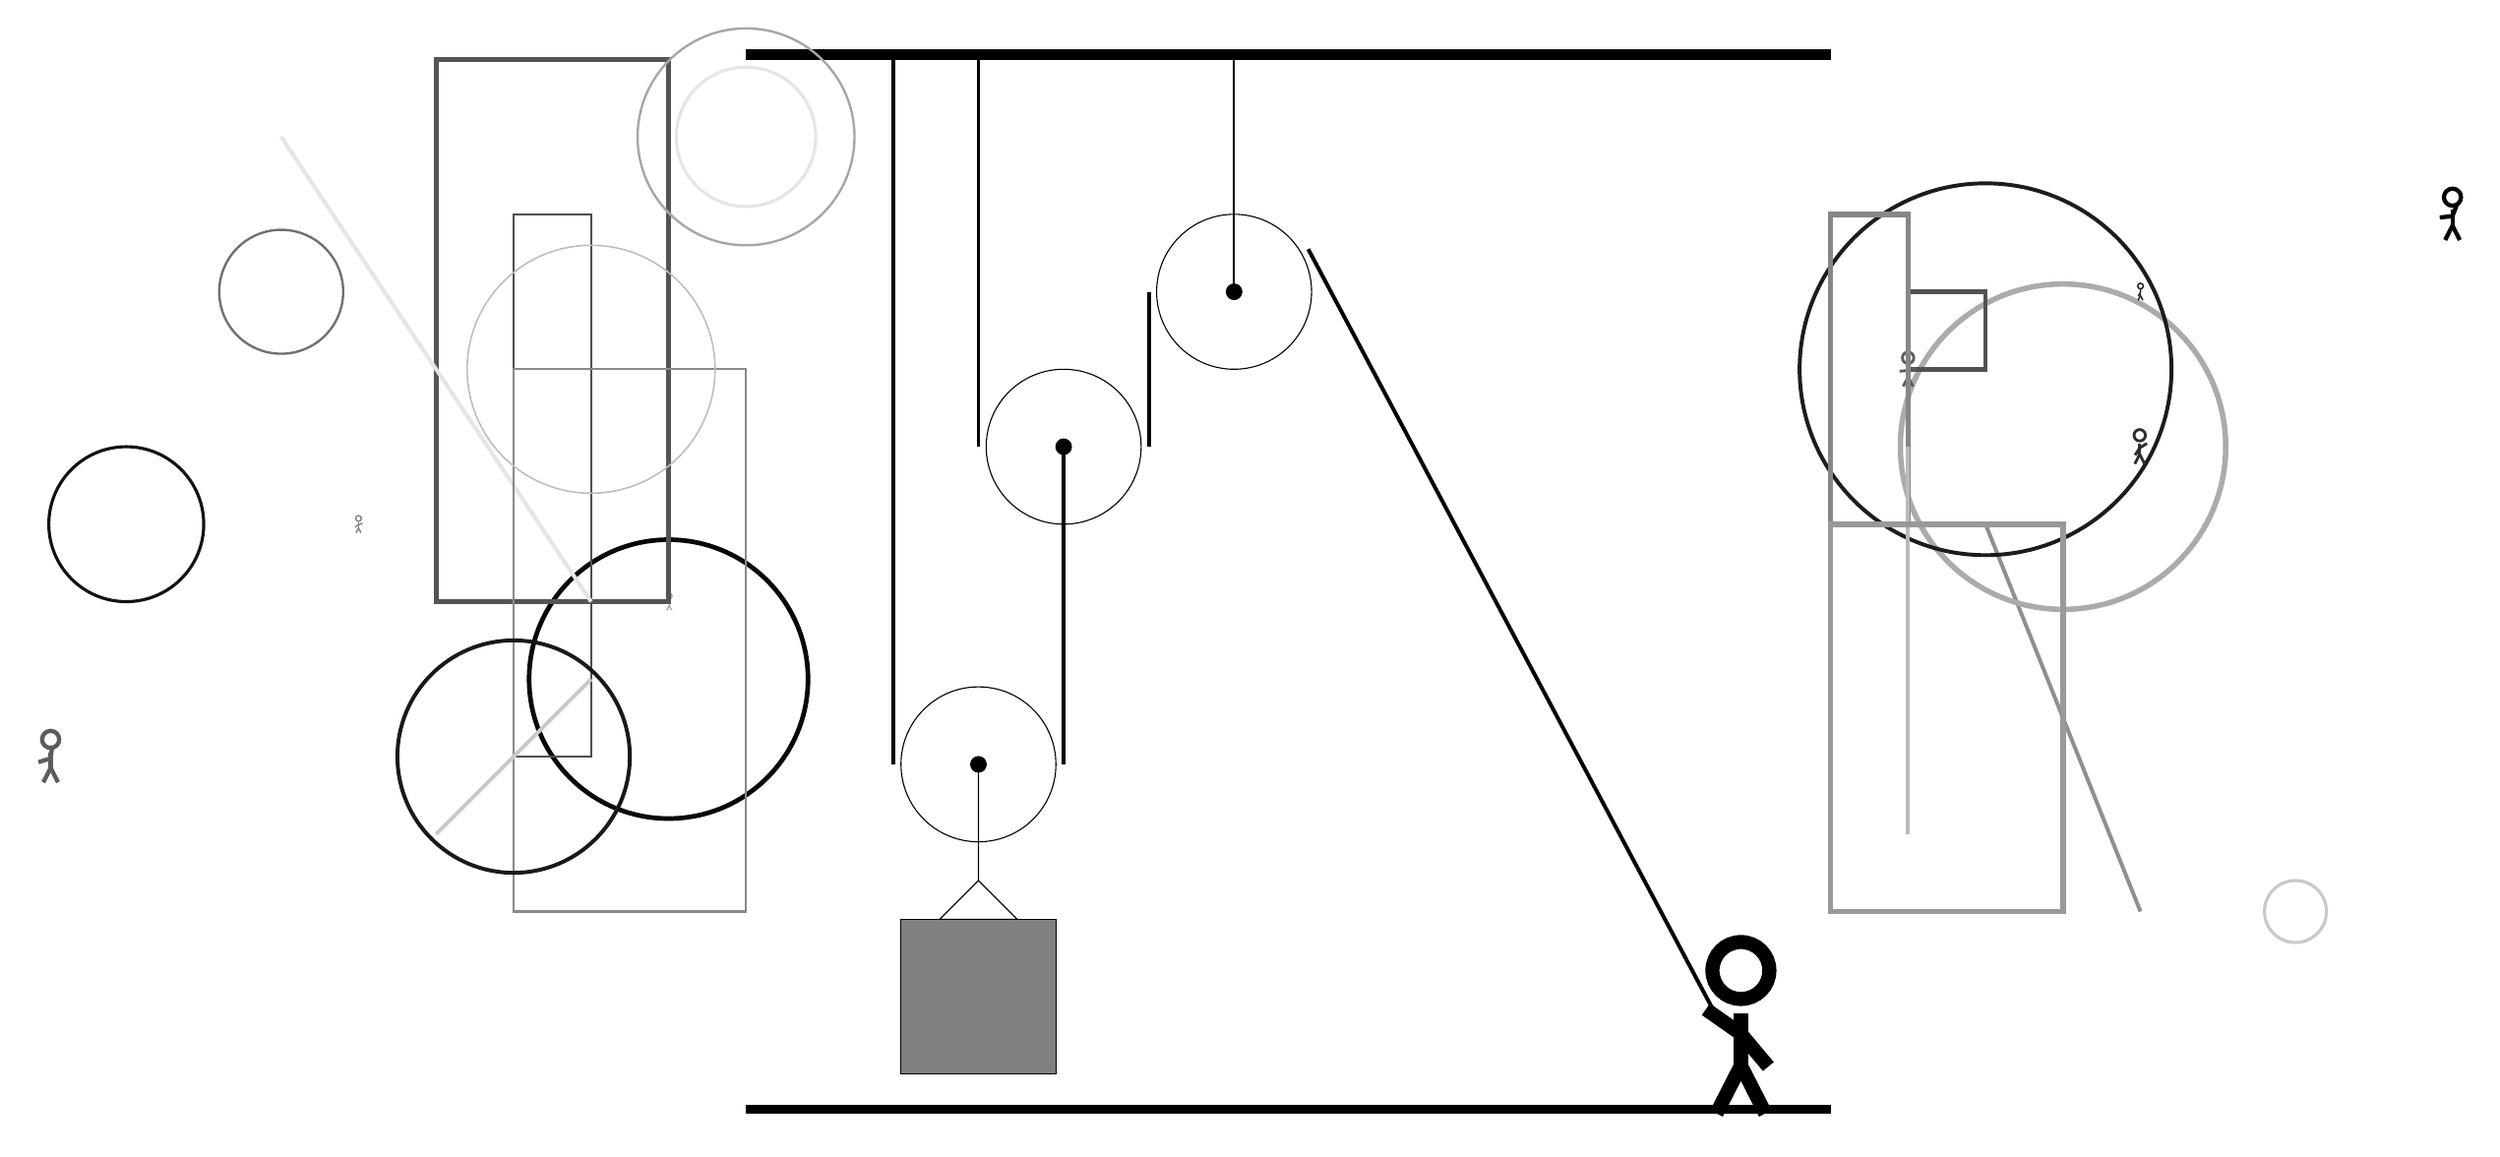
\begin{tikzpicture}
			%%%%% START %%%%%
			
			\draw[fill=black] (-2, 10) rectangle (12, 10.125);
			
			\draw (1, 0.9) circle (1);
			\draw[fill=black] (1, 0.9) circle (0.1);
			
			\draw (2.1, 5.0) circle (1);
			\draw[fill=black] (2.1, 5.0) circle (0.1);
			
			\draw (4.3, 7.0) circle (1);
			\draw[fill=black] (4.3, 7.0) circle (0.1);
			\draw[thick] (4.3, 7.0) -- (4.3, 10);
			
			\draw [line width=0.6mm, color=black!97](-3, 2) circle (1.8);
			
			\draw [line width=0.4mm, color=black!93](-10, 4) circle (1.0);
			\draw[line width=0.3mm, color=black!69] (-4, 8) rectangle (-5, 1);
			\node[line width=0.6mm, color=black!99] at (20, 8) {\Strichmaxerl[3][6][69]};
			\node[line width=0.3mm, color=black!50] at (-7, 4) {\Strichmaxerl[1][32][23]};
			
			\node[line width=0.7mm, color=black!34] at (-3, 3) {\Strichmaxerl[1][10][71]};
			
			\draw[line width=0.5mm, color=black!44](16, -1) -- (14, 4);
			
			\draw[line width=0.7mm, color=black!67] (-3, 3) rectangle (-6, 10);
			\draw[line width=0.5mm, color=black!10](-4, 3) -- (-8, 9);
			
			\draw [line width=0.7mm, color=black!33](15, 5) circle (2.1);
			\draw [line width=0.5mm, color=black!89](14, 6) circle (2.4);
			\draw[line width=0.3mm, color=black!46] (-2, 6) rectangle (-5, -1);
			\node[line width=0.2mm, color=black!64] at (-11, 1) {\Strichmaxerl[3][17][83]};
			
			\node[line width=0.3mm, color=black!82] at (16, 5) {\Strichmaxerl[2][57][32]};
			\draw [line width=0.3mm, color=black!35](-2, 9) circle (1.4);
			\draw [line width=0.4mm, color=black!10](-2, 9) circle (0.9);
			
			\draw[line width=0.6mm, color=black!68] (14, 7) rectangle (13, 6);
			\node[line width=0.5mm, color=black!64] at (13, 6) {\Strichmaxerl[2][5][9]};
			\draw [line width=0.3mm, color=black!56](-8, 7) circle (0.8);
			
			\draw[line width=0.7mm, color=black!47] (13, 4) rectangle (12, 8);
			\draw [line width=0.2mm, color=black!26](-4, 6) circle (1.6);
			\draw[line width=0.5mm, color=black!21](-4, 2) -- (-6, 0);
			
			\draw[line width=0.5mm, color=black!27](13, 0) -- (13, 5);
			\node[line width=0.6mm, color=black!87] at (16, 7) {\Strichmaxerl[1][59][87]};
			\draw[line width=0.7mm, color=black!40] (12, -1) rectangle (15, 4);
			
			\draw [line width=0.4mm, color=black!21](18, -1) circle (0.4);
			\draw [line width=0.5mm, color=black!90](-5, 1) circle (1.5);
			
			\draw (1, 0.9) -- (1, -0.6) -- (0.5, -1.1) -- (1.5, -1.1) -- (1, -0.6);
			\draw[fill=black!50] (0, -1.1) rectangle (2, -3.1);
			
			\draw[line width=0.5mm] (-0.1, 10) -- (-0.1, 0.9);
			\centerarc[line width=0.5mm](1, 0.9)(180:360:1.1);
			\draw[line width=0.5mm](2.1, 0.9) -- (2.1, 5.0);
			\draw[line width=0.5mm] (1.0, 10) -- (1.0, 5.0);
			\centerarc[line width=0.5mm](2.1, 5.0)(180:360:1.1);
			\draw[line width=0.5mm](3.2, 5.0) -- (3.2, 7.0);
			\centerarc[line width=0.5mm](4.3, 7.0)(30:180:1.1);
			\draw[line width=0.5mm] (5.257, 7.55) -- (10.5, -2.3);
			
			\node at (10.8, -2.5) {\Strichmaxerl[10][-35][-50]};
			
			\draw[fill=black] (-2, -3.5) rectangle (12, -3.6);
			
			%%%%% END %%%%%
		\end{tikzpicture}
	\end{figure}	
\end{document}